\section{extend-Beziehung}

\begin{tcolorbox}[title=extend-Beziehung]
    Die Verwendung der \code{extend}-Beziehung erlaubt die Erweiterung eines Anwendungsfalles \code{A} durch einen Anwendungsfall \code{B}.\\
    \code{A} beschreibt die Basisfunktionalität, \code{B} beschreibt die Erweiterung (s. Abbildung~\ref{fig:usecase-extend-cc}).
    Hierbei kann \code{A} alleine oder zusammen mit \code{B} ausgeführt werden (im Unterschied zur \code{include}-Beziehung: Der inkludierte Anwendungsfall wird in jedem Fall ausgeführt) (vgl.~\cite[54]{Bal05}).

    \noindent
    Bei der Verwendung einer \code{extend}-Beziehung gilt (vgl.~\cite[53]{Buh09}):

    \begin{itemize}
        \item das Verhalten eines Anwendungsfalles kann durch das Verhalten eines anderen erweitert werden
        \item die Beziehung zwischen den beteiligten Anwendungsfällen ist gerichtet
        \item spezifische Erweiterungspunkte (\textit{extension points}\footnote{
            ``ExtensionPoints may be listed in a compartment of the UseCase with the heading \textbf{extension points}.`` (\cite[642, Hervorhebung i.O.]{OMG17})
        }) geben an, an welchen Stellen der Basis-Anwendungsfall erweitert wird
        \item Bedingungen zum Auslösen des erweiterten Verhaltens wird mit angefügten Notizen spezifiziert
    \end{itemize}

    \noindent
    Bei der \code{extend}-Beziehung zeigt der Pfeil auf den zu erweiternden Anwendungsfall (\cite[218]{Oes05}), also umgekehrt zu der \code{include}-Beziehung.

\end{tcolorbox}

\begin{figure}
    \centering
    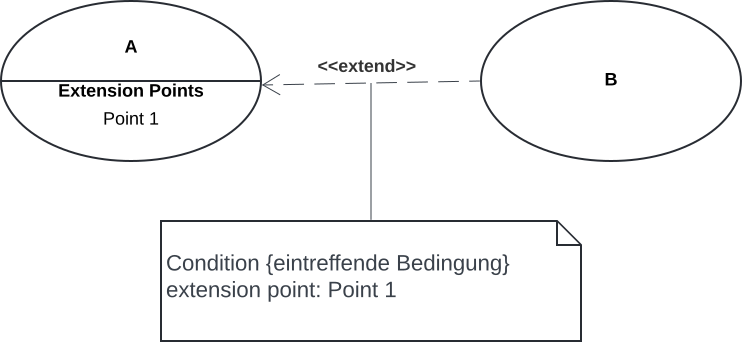
\includegraphics[scale=0.4]{part three/Anwendungsfalldiagramm/img/usecase-extend}
    \caption{Notation der extend-Beziehung. in dem Beispiel wird die der Anwendungsfall \textbf{A} durch den Anwendungsfall \textbf{B} an dem \textit{extension point} \textbf{Point 1} erweitert, der aktiviert wird, falls die in der Notiz vermerkte Bedingung zutrifft (Quelle: in Anlehnung an \cite[65, Abb. 2.8-4]{Bal05}) (Die Notizverbindung ist auch im Original durchgezogen, sollte aber gestrichelt sein, s. \cite[``Figure 7.2 Comment notation``, 22]{OMG17})}
    \label{fig:usecase-extend-cc}
\end{figure}

